\documentclass[11pt]{article}
\usepackage[margin=1in]{geometry}
\usepackage{mathpazo}
\usepackage{amsmath,amssymb}
\usepackage{microtype}
\usepackage{booktabs}
\usepackage{graphicx}
\usepackage[dvipsnames]{xcolor}
\usepackage{tikz}
\usetikzlibrary{positioning,arrows.meta,calc,fit,backgrounds}
\usepackage[most]{tcolorbox}
\usepackage{enumitem}
\usepackage{listings}
\usepackage[font=small,labelfont=bf]{caption}
\usepackage{hyperref}
\hypersetup{colorlinks=true,linkcolor=MidnightBlue,citecolor=MidnightBlue,urlcolor=MidnightBlue}
\usepackage{cleveref}
\urlstyle{tt}
\def\UrlBreaks{\do\_\do/\do.}
\newcommand{\file}[1]{\nolinkurl{#1}}
\newcommand{\code}[1]{\texttt{#1}}
\newcommand{\mhh}{m_{hh}}
\newcommand{\bw}{\boldsymbol{\omega}}
\newcommand{\bp}{\boldsymbol{p}}
\newcommand{\bx}{\boldsymbol{x}}
\newcommand{\data}{\mathcal{D}}

\definecolor{trainable}{HTML}{1B6CA8}
\definecolor{physics}{HTML}{2E933C}
\definecolor{datac}{HTML}{7B4EA3}
\definecolor{warn}{HTML}{C0392B}

\newtcolorbox{keyidea}[1][]{enhanced,breakable,colback=physics!6,colframe=physics!70!black,
  fonttitle=\bfseries,title={#1},boxrule=0.6pt,arc=2pt,left=6pt,right=6pt}
\newtcolorbox{aside}[1][]{enhanced,breakable,colback=trainable!5,colframe=trainable!70!black,
  fonttitle=\bfseries,title={#1},boxrule=0.6pt,arc=2pt,left=6pt,right=6pt}
\newtcolorbox{assume}[1][]{enhanced,breakable,colback=datac!5,colframe=datac!70!black,
  fonttitle=\bfseries,title={#1},boxrule=0.6pt,arc=2pt,left=6pt,right=6pt}
\newtcolorbox{watch}[1][]{enhanced,breakable,colback=warn!5,colframe=warn!70!black,
  fonttitle=\bfseries,title={#1},boxrule=0.6pt,arc=2pt,left=6pt,right=6pt}
\setlist{itemsep=2pt,topsep=3pt}
\setlength{\emergencystretch}{3em}

\lstset{language=Python, basicstyle=\ttfamily\small, columns=fullflexible,
  keepspaces=true, commentstyle=\color{physics!70!black}\itshape,
  keywordstyle=\color{trainable!90!black}\bfseries, stringstyle=\color{datac},
  showstringspaces=false, frame=single, rulecolor=\color{gray!40},
  backgroundcolor=\color{gray!3}, xleftmargin=4pt, xrightmargin=4pt,
  aboveskip=6pt, belowskip=6pt}

\title{\textbf{Bayesian neural networks}\\[4pt]
\large Hamiltonian Monte Carlo after Radford Neal}
\date{November 12, 2026}

\author{Harrison B. Prosper}
\begin{document}
\maketitle

\begin{abstract}
\noindent
This note describes an ML model-agnostic Python module, \code{hmc}, written by \code{Claude Pro}, which implements \emph{Bayesian neural networks} (BNN) 
following closely the approach of Radford
Neal~\cite{neal1996,neal2011}. Machine learning models trained using gradient descent 
provide a \emph{point estimate} of the model parameters, that is, a single best-fit point. 
This is analogous to maximimum likelihood, and in some cases the procedure is identical to 
maximum likelihood. A BNN is
an ensemble of parameter points sampled from the posterior density of the parameters of an ML
model
given the training data. The points are sampled using Hamiltonian Monte Carlo (HMC)  and the module
uses PyTorch to compute gradients. Each sampled vector of parameters is saved 
to its own \file{params_NNNN.pth} file in a run folder. A companion class, \code{BNN},
reads those files back and computes the posterior mean of the network output, its
standard deviation, quantiles and intervals. 
\end{abstract}

\tableofcontents

% ===========================================================================
\section{The Bayesian neural network}
\label{sec:bnn}

\subsection{From a point estimate to an ensemble}

Most machine learning models are trained, that is, fitted by finding  one parameter vector $\bw^*$ by minimizing the empirical
risk. Neal's
idea~\cite{neal1996} is to treat $\bw$ like any other unknown parameter in a
Bayesian analysis. Bayes' theorem gives the posterior density
\begin{equation}
  p(\bw \mid \data) = \frac{p(\data \mid \bw)\, \pi(\bw)}{p(\data)},
  \qquad \data = \{(\bx_i, t_i),\ i = 1,\ldots,N\},
  \label{eq:bayes}
\end{equation}
where $p(\data \mid \bw)$ is the likelihood, $\pi(\bw)$ the prior and $t_i$  are the targets. The prediction at a new point $\bx$ is an
ensemble of predictions from which various summaries can be computed, for example, 
 the posterior mean,
\begin{equation}
  \bar f(\bx) = \int f(\bx; \bw)\, p(\bw \mid \data)\, d\bw
  \;\approx\; \frac{1}{K} \sum_{k=1}^{K} f(\bx; \bw_k),
  \qquad \bw_k \sim p(\bw \mid \data).
  \label{eq:mean}
\end{equation}
The sampling of the posterior density is performed using the HMC sampler  and each sampled point
is stored
in \file{params_NNNN.pth} files. Other summaries that can be approximated from the ensemble
of parameters points are the standard deviation of
$f(\bx; \bw)$ and its quantiles.

\subsection{The prior}
\label{sec:prior}
Every Bayesian analysis requires the specification of a prior.
Neal groups the parameters of a network by role and gives each group $g$ its own
Gaussian prior, whose width is itself unknown~\cite[ch.~2 and 3]{neal1996}:
\begin{equation}
  \bw_g \mid \tau_g \sim \mathcal{N}\!\left(0,\ \tau_g^{-1} I\right), \qquad
  \tau_g \sim \text{Gamma}(\alpha_g, \beta_g).
  \label{eq:prior}
\end{equation}
Here $\tau_g$ is the \emph{precision} (the inverse variance) of group $g$, and
$\alpha_g, \beta_g$ are the shape and rate of its Gamma prior. In principle, such a
\emph{hierarchical} prior allows the data to determine the typical size of the weights of each layer. 
The Gamma prior is an example of a \emph{hyperprior}, that is, a prior that determines some
parameters of 
a prior. The parameters of a hyperprior are referred to as \emph{hyperparameters}.
%\begin{table}[h]
%\centering\small
%\begin{tabular}{llrl}
%\toprule
%group (PyTorch name) & role & size & default prior scale $\sigma_g$\\
%\midrule
%\code{P.0.weight}, \code{P.0.bias} & input ($\mhh$) $\to$ hidden 1 & 25 + 25 & $1/\sqrt{1}$, 1\\
%\code{P.2.weight}, \code{P.2.bias} & hidden 1 $\to$ hidden 2 & 625 + 25 & $1/\sqrt{25}$, 1\\
%\quad$\vdots$ & \quad$\vdots$ (hidden layers 3 to 6) & & \\
%\code{P.12.weight}, \code{P.12.bias} & hidden 6 $\to$ 23 outputs ($\tanh$) & 575 + 23 & $1/\sqrt{25}$, 1\\
%\code{Q.weight}, \code{Q.bias} & $\mhh \to$ 23 exponents & 23 + 23 & 1, 1\\
%\midrule
%16 groups & & 3,944 & \\
%\bottomrule
%\end{tabular}
%\caption{The parameter groups of \code{HEFTNet}. The indices 0, 2, \ldots, 12 are
%the positions of the \code{nn.Linear} layers inside \code{nn.Sequential}; the odd
%positions hold the activation functions, which have no parameters. The proposed
%default prior mean of $\tau_g$ is $1/\sigma_g^2$, with $\sigma_g = 1/\sqrt{\text{fan-in}}$
%for weights (Neal's scaling, which keeps the prior on the function sensible as the
%width grows~\cite[ch.~2]{neal1996}) and $\sigma_g = 1$ for biases.}
%\label{tab:groups}
%\end{table}

\begin{aside}[The hyperparameters can be sampled exactly (Gibbs sampling)]
Given the current weights $\bw_g$ (with $n_g$ elements), the density of $\tau_g$ is
\[
p(\tau_g \mid \bw_g) \propto
\underbrace{\tau_g^{n_g/2} e^{-\tau_g \lVert\bw_g\rVert^2/2}}_{\text{Gaussian prior on }\bw_g}
\;\underbrace{\tau_g^{\alpha_g - 1} e^{-\beta_g \tau_g}}_{\text{Gamma prior}}
= \tau_g^{(\alpha_g + n_g/2) - 1}\, e^{-(\beta_g + \lVert\bw_g\rVert^2/2)\,\tau_g},
\]
which is again a Gamma density, with shape $\alpha_g + n_g/2$ and rate
$\beta_g + \lVert\bw_g\rVert^2/2$. (A prior with this property is called
\emph{conjugate}.) A new $\tau_g$ can therefore be drawn exactly with
\code{torch.distributions.Gamma}, with no tuning and no rejection. Neal's software
alternates such Gibbs draws of the hyperparameters with HMC updates of the
weights~\cite{neal1996}; we do the same.
\end{aside}

\subsection{The likelihood}
\label{sec:likelihood}

In principle, we start with a statistical model, $p(x \mid \omega)$, of a potential instance of training data $x$ into which actaul training data $t$ are inserted thereby yielding the likelihood, or, what is more useful, the negative log-likelihood $\ell(t \mid \theta) = -\log p(t \mid \theta)$. In practice, however, we do not know the functional form of $\ell(t \mid \theta)$. Therefore, we introduce a model $f(x; \omega)$ and write $\ell(t \mid f)$.
 Three choices will be offered through a switch,
\code{LIKELIHOOD}:
\begin{center}
\small
\begin{tabular}{lllp{0.36\textwidth}}
\toprule
\code{LIKELIHOOD} & $-\log p(t_i \mid f_i)$ & counterpart & noise parameter\\
\midrule
\code{'laplace'} (default) & $\lvert t_i - f_i\rvert / b + \log 2b$ & L1 loss
  & one scale $b$ (pb), Gibbs-sampled (inverse-Gamma)\\
\code{'gaussian'} & $(t_i - f_i)^2 / 2s^2 + \log s$ & MSE loss
  & one variance $s^2$, Gibbs-sampled (inverse-Gamma)\\
\code{'poisson'} (experimental) & $(t_i - f_i)^2 / 2\sigma_i^2$ & CHI2 loss
  & none: $\sigma_i^2 = w_j t_i$ known from the event count\\
\bottomrule
\end{tabular}
\end{center}

\noindent The Gibbs draw of the noise scale works exactly as for $\tau_g$. For the
Laplace likelihood with an inverse-Gamma prior $b \sim \text{InvGamma}(\alpha_b, \beta_b)$,
\[
  b \mid \bw, \data \sim \text{InvGamma}\Big(\alpha_b + N,\ \ \beta_b + \sum_i \lvert t_i - f_i\rvert\Big),
\]
and for the Gaussian, $s^2 \mid \bw, \data \sim \text{InvGamma}(\alpha_s + N/2,\ \beta_s + \sum_i (t_i - f_i)^2/2)$.

% ===========================================================================
\section{Hamiltonian Monte Carlo}
\label{sec:hmc}

\subsection{The idea}

Write the posterior as a Boltzmann distribution, $p(\bw \mid \data) \propto
e^{-U(\bw)}$, with the \emph{potential energy}
\begin{equation}
  U(\bw) = -\log p(\data \mid \bw) - \log \pi(\bw \mid \tau).
\end{equation}
HMC~\cite{duane1987,neal2011} treats $\bw$ as the position of a fictitious particle
moving in the potential $U$ with a fictitious momentum $\bp$, one component
per parameter, with kinetic energy $K(\bp) = \tfrac12 \bp^{\mathsf T} M^{-1} \bp$,
where $M$ is a ``mass matrix''. The joint density of $(\bw, \bp)$ is
$\propto e^{-H(\bw, \bp)}$ with the Hamiltonian $H = U + K$. By construction, $\bw$ and $\bp$ are independent and
the marginal of $\bw$ is the desired posterior density. Each HMC update comprises three steps:

\begin{enumerate}
  \item \textbf{Kick.} Sample a momentum, $\bp \sim \mathcal{N}(0, M)$.
  \item \textbf{Glide.} Follow Hamilton's equations, $d\bw/ds = M^{-1}\bp$,
    $d\bp/ds = -\nabla U(\bw)$, for a fictitious time $L\varepsilon$, using $L$
    \emph{leapfrog} steps of size $\varepsilon$:
    \begin{align*}
      \bp &\leftarrow \bp - \tfrac{\varepsilon}{2}\, \nabla U(\bw) && \text{(half step in momentum)}\\
      \bw &\leftarrow \bw + \varepsilon\, M^{-1}\bp && \text{(full step in position)}\\
      \bp &\leftarrow \bp - \tfrac{\varepsilon}{2}\, \nabla U(\bw) && \text{(half step in momentum)}
    \end{align*}
    (consecutive half steps in momentum are merged, so each leapfrog step costs one
    gradient).
  \item \textbf{Accept or reject.} Exact dynamics would conserve $H$,  however, the leapfrog algorithm does
    so only approximately. But if the end point $(\bw', \bp')$ is accepted with
    probability $\min\{1, e^{-\Delta H}\}$, $\Delta H = H(\bw', \bp') - H(\bw, \bp)$ and rejected otherwise, thereby leaving the particle at $\bw$, the procedure corrects for this error exactly on average. 
\end{enumerate}

\noindent \Cref{fig:hmc} shows why this is worth the trouble. Neural-network
posterior densities are full of long, narrow ridges. A random-walk sampler must take steps
no larger than the width of the ridge, so it diffuses along it slowly. An HMC
trajectory follows the ridge, because the gradient keeps pushing it back into the
valley, and in one update travels a distance comparable to the length of the ridge.
Along the way $U$ and $K$ exchange energy while $H$ stays nearly constant, so the
acceptance probability stays high.

\begin{figure}[h]
\centering
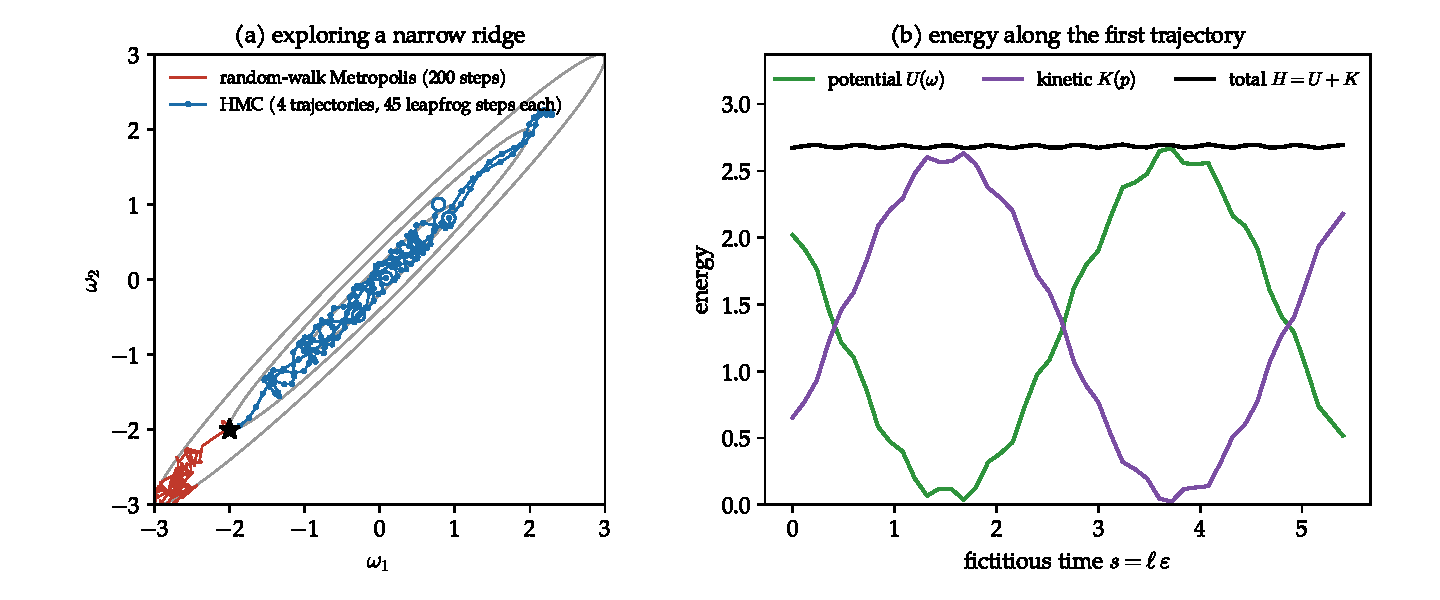
\includegraphics[width=\textwidth]{fig_hmc.pdf}
\caption{(a) Sampling a Gaussian with correlation 0.98, starting at the star.
200 random-walk Metropolis steps (red) barely move, while each of four HMC
trajectories (blue; open circles are the end points) crosses much of the ridge.
(b) Along one trajectory, potential and kinetic energy trade places while the total
energy $H$ is conserved to about 1\%, so the end point is almost always accepted.}
\label{fig:hmc}
\end{figure}

\begin{aside}[Why the result is exactly the posterior, and not an approximation]
The leapfrog map has two properties that hold whatever $\varepsilon$ is: it is
\emph{reversible} (run it again after flipping the sign of $\bp$ and you return to
the start) and it \emph{preserves volume} in $(\bw, \bp)$ space (each of the three
sub-steps is a shear, which changes one set of coordinates by an amount that depends
only on the other set). With these two properties, the accept/reject step makes the
chain satisfy detailed balance with respect to $e^{-H}$ exactly~\cite{neal2011}.
A large $\varepsilon$ only lowers the acceptance rate; it does not bias the samples.
Neither property needs $U$ to be smooth, so the kinks of $\lvert t - f\rvert$ and of
the ReLU are allowed; they merely make $\Delta H$ a little larger.
\end{aside}

\subsection{Tuning: step size, trajectory length, mass matrix}
\label{sec:tuning}

The HMC class has three settings, which are adjusted during a \emph{warm-up} phase, whose
samples are discarded. The settings are then frozen because changing them while sampling would
break the Markov property.

\begin{itemize}
  \item \textbf{Step size $\varepsilon$.} Too large: $\Delta H$ is large and most
    trajectories are rejected. Too small: each trajectory moves a short distance.
    During warm-up, $\varepsilon$ is adjusted by \emph{dual averaging}~\cite{hoffman2014}
    so that the average acceptance rate reaches a target (default 0.8): raised when
    the acceptance is above target, lowered when below, with an averaging that makes
    it settle. In the sampling phase each trajectory uses $\varepsilon$ times a random
    factor between 0.9 and 1.1 (``jitter''), as Neal recommends, to avoid trajectories
    that happen to return to their start.
  \item \textbf{Number of leapfrog steps $L$.} Fixed by the user (switch
    \code{N\_LEAPFROG}), also with a small random jitter. The diagnostics of
    \cref{sec:diagnostics} tell whether it is long enough.
  \item \textbf{Mass matrix $M$.} The leapfrog step in $\bw$ is $\varepsilon M^{-1}\bp$.
    If some parameters are far more tightly constrained than others, one $\varepsilon$
    cannot suit all of them. Setting $M^{-1}$ to the posterior \emph{variance} of each
    parameter, estimated from the second half of the warm-up, rescales every parameter
    to unit width~\cite{neal2011}. 
\end{itemize}

\begin{assume}[What HMC requires of the problem]
\begin{enumerate}
  \item $U(\bw)$ and $\nabla U(\bw)$ can be computed (almost everywhere) for any $\bw$.
    PyTorch autograd supplies the gradient.
  \item The model is a \emph{deterministic} function of its inputs and parameters:
    no dropout and no batch normalisation. The module checks this.
  \item \textbf{Every gradient uses all training data.} A gradient from a random
    mini-batch is noisy, and noisy gradients destroy the conservation of $H$ on which
    the accept/reject step relies. (Stochastic-gradient variants exist~\cite{chen2014},
    but they sample the posterior only approximately.)
    The sum over data will be computed in chunks to bound memory; the sum of the
    chunks is exact.
\end{enumerate}
\end{assume}

% ===========================================================================
\section{Applying HMC}
\label{sec:heftnet}

\subsection{Warm start}
\label{sec:warm}

Neal starts his chains from small random weights and lets them find the region of
high posterior density. The recommendation is 
to start from the parameters of a model trained with the L1 loss. The hyperparameters start at
values computed from those weights: $\tau_g = n_g/\lVert\bw_g\rVert^2$, and $b$
equal to the mean absolute residual. A short warm-up then lets the chain settle into
the posterior proper. Setting \code{WARM\_START = None} reproduces Neal's
start from the prior, for comparison.

\subsection{What can go wrong and what is done about it}
\label{sec:cost}


\begin{watch}
%[What can go wrong, and what the module does to mitigate problems]
\begin{enumerate}
  \item \textbf{Bad conditioning.} Neural-network posteriors have directions that are
    constrained a million times more tightly than others. A diagonal mass matrix
    removes differences of scale between parameters but not correlations among them.
    If the acceptance is good but the samples are strongly autocorrelated, $L$ must
    grow. Large studies of full-data HMC for networks~\cite{izmailov2021} needed long
    trajectories; we should expect the same.
  \item \textbf{Precision.} $U$ is a sum of a large number of terms of order 1 or more, while the
    accept/reject step needs $\Delta H$ to about 0.01. In single precision (about 7
    digits) the sum would likely not be computed with sufficient accuracy. The model will run in single
    precision, but $U$, $H$ and the chunk sums will be accumulated in double precision.
  \item \textbf{Divergences.} If $\Delta H$ exceeds 1,000, the trajectory has gone
    unstable. It is rejected, counted,
    and reported; many divergences mean $\varepsilon$ is too large.
  \item \textbf{Symmetries.} Machine learning models typically have an exponentially large number of equivalent minima in the loss landscape. This is why it is even remotely possible to find good local minima: there are an astronomically large number of equivalent minima to choose from! For example, permuting the hidden units of a layer, or rescaling a
    ReLU unit's input weights by $c$ and its output weights by $1/c$, leaves $f$
    unchanged. Therefore, individual weights need not converge, and are not
    monitored; only quantities that matter are monitored, $U$, the hyperparameters and predictions
    at chosen input points.
\end{enumerate}
\end{watch}

% ===========================================================================
\section{The module \texttt{hmc.py}}
\label{sec:module}

\subsection{Design}

\Cref{fig:arch} shows the pieces and how data flow between them. Each piece is a
small class with one job. 

\begin{figure}[h]
\centering
\resizebox{\textwidth}{!}{%
\begin{tikzpicture}[
  font=\small, >={Stealth[length=2.2mm]},
  box/.style={draw, rounded corners=2pt, thick, align=center, inner sep=3pt,
              minimum height=12mm, text width=30mm},
  usr/.style={box, fill=datac!8, draw=datac!80!black},
  mod/.style={box, fill=trainable!10, draw=trainable!80!black},
  res/.style={box, fill=physics!10, draw=physics!80!black, text width=36mm},
]
\node[usr] (model) at (0, 2.2)  {\code{HEFTNet()}\\\footnotesize any \code{nn.Module}};
\node[usr] (dat)   at (0, 0)    {training data\\\footnotesize tensors $X$, $t$};
\node[usr] (lik)   at (0, -2.2) {\code{LaplaceLikelihood}\\\footnotesize or Gaussian, Poisson};
\node[mod] (view)  at (4.2, 2.2) {\code{ParameterView}\\\footnotesize finds the 16 groups;\\\footnotesize model $\leftrightarrow$ flat $\bw$};
\node[mod] (prior) at (4.2, -2.2){\code{HierarchicalPrior}\\\footnotesize Neal's $\tau_g$; Gibbs};
\node[mod] (post)  at (8.4, 0)   {\code{Posterior}\\\footnotesize $U(\bw)$, $\nabla U(\bw)$\\\footnotesize (autograd, chunks)};
\node[mod] (hmc)   at (12.6, 0)  {\code{HMC}\\\footnotesize leapfrog, accept,\\\footnotesize warm-up, Gibbs};
\node[res] (run)   at (12.6, 2.6){\file{runs/BNN_laplace/}\\\footnotesize \file{samples/params_*.pth}\\\footnotesize trace, state};
\node[res] (bnn)   at (12.6, -2.6){\code{BNN}\\\footnotesize mean, std,\\\footnotesize quantiles, intervals};
\draw[->, thick] (model) -- (view);
\draw[->, thick] (view) -- (post);
\draw[->, thick] (dat) -- (post);
\draw[->, thick] (lik) -- (post);
\draw[->, thick] (prior) -- (post);
\draw[->, thick] (view) -- (prior);
\draw[->, thick] (post) -- (hmc);
\draw[->, thick] (hmc) -- node[right, font=\footnotesize]{writes} (run);
\draw[->, thick] (run.east) -- ++(0.6,0) |- node[pos=0.25, right, font=\footnotesize]{reads} (bnn.east);
\end{tikzpicture}}
\caption{The classes of \file{hmc.py} (blue), what the user provides (purple) and what
the sampler produces (green).}
\label{fig:arch}
\end{figure}

\subsection{Finding the parameters automatically}
\label{sec:view}

Every PyTorch model is an \code{nn.Module}, and every \code{nn.Module} can list its
own parameters, with their names, through \code{named\_parameters()}. That is all
\code{ParameterView} needs; it never looks inside the model's code. The module  finds the relevant groups of parameters by name and shape,
and by default makes each tensor a group of Neal's prior. It also provides the two
conversions HMC needs: from the model's tensors to one flat vector $\bw$ of 
numbers (the ``position'') and back. Here is a sketch of the code:

\begin{lstlisting}
class ParameterView:
    def __init__(self, model):
        self.model = model
        self.names, self.params = [], []
        # named_parameters() walks through every sub-module of the model and
        # yields (name, tensor) pairs, e.g. ('P.0.weight', tensor of shape
        # [25, 1]), ('P.0.bias', tensor of shape [25]), ..., ('Q.bias', [23]).
        for name, p in model.named_parameters():
            if p.requires_grad:          # skip parameters frozen by the user
                self.names.append(name)
                self.params.append(p)
        # numel() = number of elements of a tensor, e.g. 25*25 = 625.
        self.sizes = [p.numel() for p in self.params]
        # where each tensor sits inside the flat vector: a list of slices,
        # e.g. 'P.0.weight' -> slice(0, 25), 'P.0.bias' -> slice(25, 50), ...
        ends = np.cumsum(self.sizes)
        self.slices = [slice(e - n, e) for e, n in zip(ends, self.sizes)]

    def get(self):
        # Copy all parameters into ONE flat vector (the HMC "position").
        # detach() cuts the link to the autograd history; clone() makes an
        # independent copy, so changing it does not change the model.
        return parameters_to_vector(self.params).detach().clone()

    def set(self, w):
        # Write a flat vector back into the model's tensors, in place.
        vector_to_parameters(w, self.params)
\end{lstlisting}

\noindent The gradient $\nabla U$ is obtained the same way: compute $U$ with the
model's parameters set to $\bw$, call \code{U.backward()}, and collect each
parameter's \code{.grad} into a flat vector in the same order. Groups can also be
chosen coarser (\code{grouping='all'}: one $\tau$ for every parameter) or by an
explicit dictionary from names to groups.

\paragraph{What a model must satisfy.} It is a \code{torch.nn.Module}; its
\code{forward} takes a tensor of inputs and returns one prediction per row; it has no
dropout or batch-normalisation layers (\code{ParameterView} inspects
\code{model.modules()} and stops with an explanation if it finds one); and it can be
rebuilt by calling its class with no arguments, so that \code{BNN} can recreate it. The 
\code{FCCN} class in module \code{drwho} satisfies all four
requirements if dropout is omitted.

\subsection{The classes and their methods}

\begin{center}
\small
\begin{tabular}{p{0.24\textwidth}p{0.70\textwidth}}
\toprule
class & main methods\\
\midrule
\code{ParameterView} & \code{get()}, \code{set(w)}, \code{grad()}, \code{groups},
  \code{summary()} (prints the table of groups)\\
\code{HierarchicalPrior} & \code{neg\_log(w)} $= \sum_g \tau_g\lVert\bw_g\rVert^2/2$;
  \code{gibbs(w)}: new $\tau_g$; \code{from\_weights(w)}: initial $\tau_g$\\
\code{LaplaceLikelihood}, \code{GaussianLikelihood}, \code{PoissonLikelihood} &
  \code{neg\_log(f, t)}; \code{gibbs(residuals)}: new noise scale (not for Poisson);
  \code{sample(f)}: simulated data, for predictive bands\\
\code{Posterior} & \code{U(w)}, \code{U\_and\_grad(w)}: sum over chunks of rows, in
  double precision; \code{time\_gradient()}\\
\code{HMC} & \code{run(n\_warmup, n\_samples, thin)}; \code{resume()};
  \code{acceptance\_rate()}; internally \code{leapfrog()}, \code{trajectory()},
  \code{adapt\_step\_size()}, \code{adapt\_mass()}\\
\code{BNN} & \code{predict(x)} $\to$ tensor $[K, N]$; \code{mean(x)}, \code{std(x)},
  \code{quantiles(x, q)}, \code{interval(x, cl)}, \code{predictive(x)} (adds the
  likelihood noise), \code{apply(fn, x)} (any function of a model, e.g.\ the
  coefficient functions \code{model.coeffs}), \code{len(bnn)}\\
functions & \code{autocorrelation(y)}, \code{ess(y)} (effective sample size),
  \code{rhat(chains)} (Gelman--Rubin)\\
\bottomrule
\end{tabular}
\end{center}

\noindent For sample with a large number of points, \code{mean} and
\code{std} are accumulated one sample at a time (Welford's running formulae), so the
$K \times N$ table of predictions is never held in memory. A typical use case:
\begin{lstlisting}
from drwho import hmc
from dihiggs import heftnet as NN

bnn = hmc.BNN(NN.HEFTNet, 'runs/BNN_laplace')  # reads every params_NNNN.pth
mu  = bnn.mean(x)                  # posterior mean of sigma, one per row of x
sd  = bnn.std(x)                   # its posterior standard deviation
lo, hi = bnn.interval(x, cl=0.68)  # central 68% credible interval
A   = bnn.apply(lambda m, x: m.coeffs(x[:, 0]), x)  # samples of a_i(m_hh)
\end{lstlisting}

\subsection{The run folder}
\label{sec:runfolder}

\begin{center}
\small
\begin{tabular}{p{0.38\textwidth}p{0.56\textwidth}}
\toprule
file & contents\\
\midrule
\file{runs/BNN_laplace/dihiggs_config.yaml} & every setting (\code{drwho} \code{Config}),
  the warm-start file and the training file's SHA-256, as in \file{heft_train}\\
\file{dihiggs_hmc_trace.csv} & one row per trajectory: iteration, phase (warm-up or
  sampling), accepted?, $\Delta H$, $U$, $\varepsilon$, $L$, $b$, $\tau_1 \ldots \tau_{16}$\\
\file{dihiggs_hmc_state.pth} & checkpoint, rewritten every few minutes: current $\bw$,
  $\tau$, $b$, $\varepsilon$, $M$, iteration, random-number-generator states\\
\file{samples/params_0001.pth}, \ldots & one sampled parameter set each, a plain
  \code{state\_dict}, readable by \code{HEFTNet().load(file)}\\
\file{samples/index.csv} & for each sample: file name, iteration, $U$, $b$, $\tau_g$\\
\bottomrule
\end{tabular}
\end{center}

\noindent A sample is about 16~kB, so 1,000 samples take 16~MB. Because of the
checkpoint, a run interrupted by Colab, a time limit on the RTX~5090 cluster, or a
closed laptop lid continues with \code{sampler.resume()} from where it stopped, and
the result is the same as an uninterrupted run with the same seed. With
\code{N\_CHAINS} $> 1$, each chain gets its own sub-folder, \file{chain_1/},
\file{chain_2/}, \ldots, and its own seed; \code{BNN} pools them.

% ===========================================================================

% ===========================================================================
\section{Validation}
\label{sec:validation}

\subsection{The sampler on problems with known answers}

\file{code/hmc_toy.ipynb} (seconds on a CPU) runs:
\begin{enumerate}
  \item \textbf{Bayesian linear regression}, a ``network'' with one linear layer, a
    Gaussian prior of fixed precision and Gaussian noise of known variance. The posterior
    is then Gaussian with a mean and covariance that can be written down. The sampled
    means and covariances must agree with them within their Monte Carlo errors
    (computed from the effective sample size). This tests the leapfrog integrator, the
    accept/reject step, the mass matrix and the bookkeeping of \code{ParameterView}.
  \item \textbf{Neal's one-dimensional example}~\cite{neal1996}: a small network fitted
    to noisy points of a smooth curve on part of an interval, with the hierarchical
    prior and Gibbs updates switched on. The posterior band should hug the data where
    there are data and widen outside. This is a visual check of the whole machinery,
    and a good teaching example.
\end{enumerate}

\subsection{Diagnostics}
\label{sec:diagnostics}

\begin{itemize}
  \item \textbf{Acceptance rate} in the sampling phase between about 0.6 and 0.9, and
    no (or very few) divergences.
  \item \textbf{Stationarity}: the traces of $U$, $b$ and the $\tau_g$ show no drift
    after warm-up.
  \item \textbf{Mixing}: the autocorrelation of $U$, and of the prediction at a handful
    of monitor input points; we aim for a sample size of at least 100.
  \item \textbf{Several chains}, if run: Gelman--Rubin $\hat R < 1.05$ for the same
    quantities.
\end{itemize}



% ===========================================================================
\begin{thebibliography}{9}
\bibitem{neal1996} R.~M.~Neal, \emph{Bayesian Learning for Neural Networks}, Lecture
  Notes in Statistics 118, Springer (1996).
\bibitem{neal2011} R.~M.~Neal, ``MCMC using Hamiltonian dynamics'', in \emph{Handbook of
  Markov Chain Monte Carlo}, eds.\ S.~Brooks \emph{et al.}, Chapman \& Hall/CRC (2011),
  arXiv:1206.1901.
\bibitem{duane1987} S.~Duane, A.~D.~Kennedy, B.~J.~Pendleton and D.~Roweth, ``Hybrid Monte
  Carlo'', Phys.\ Lett.\ B \textbf{195} (1987) 216.
\bibitem{hoffman2014} M.~D.~Hoffman and A.~Gelman, ``The No-U-Turn sampler: adaptively
  setting path lengths in Hamiltonian Monte Carlo'', J.\ Mach.\ Learn.\ Res.\ \textbf{15}
  (2014) 1593.
\bibitem{izmailov2021} P.~Izmailov, S.~Vikram, M.~D.~Hoffman and A.~G.~Wilson, ``What are
  Bayesian neural network posteriors really like?'', ICML 2021, arXiv:2104.14421.
\bibitem{chen2014} T.~Chen, E.~B.~Fox and C.~Guestrin, ``Stochastic gradient Hamiltonian
  Monte Carlo'', ICML 2014, arXiv:1402.4102.
\bibitem{wenzel2020} F.~Wenzel \emph{et al.}, ``How good is the Bayes posterior in deep
  neural networks really?'', ICML 2020, arXiv:2002.02405.
\end{thebibliography}

\end{document}
